% Physiology
\noindent \textbf{Earmolds reduced spectral information available for vertical sound localization}\\
Application of silicone molds to the Pinnae altered spectral cues across the measured 4-16 kHz band (Fig. 2 A - C). Both sets of earmolds had a similar effect in reducing the prominent spectral notch situated in the 5-12 kHz band and the spectral peaks to its flanks. Similar effects have been observed in previous studies using earmolds to modify spectral cues (Trapeau, Schönwiesner 2015, Carlile 2014, Hofman 1998). Comparing the VSI of modified ears to participants’ free ears showed a reduction of vertical spectral information (VSI) available for elevation discrimination in the 5.3-11.7 kHz octave band (one-tailed Wilcoxon signed rank test; VSI free ears: 0.61 +/- 0.04, VSI earmolds 1: 0.45 +/- 0.05, p = 0.003, VSI earmolds 2: 0.39 +/- 0.04, p = 0.004). As expected, the VSI of the left and right ear without molds were correlated in this band (Spearman correlation of left ear and right ear VSI; R = 0.55, p = 0.035). This correlation persisted after the earmolds were applied but was not significant for the second set of molds (earmolds 1: R = 0.56, p = 0.035, earmolds 2: R = 0.53, p = 0.064). Figure 4 shows the VSI of all participants with free ears and both sets of earmolds.\\

\end{multicols} %%% figure 1
\begin{figure}[hb]
\floatbox[{\capbeside\thisfloatsetup{capbesideposition={left,top},capbesidewidth=5cm}}]{figure}[\FBwidth]
{\caption{A test figure with its caption side by side}\label{fig:test}}
{\includegraphics[width=13cm]{../Results/figures/hrtf_compare/hrtf_compare}}
\end{figure}
\begin{multicols}{2}
\noindent % prevent indent

\noindent\textbf{Modified pinna shapes were within the physiological range}\\
To confirm that spectral changes induced by the earmolds were physiologically plausible, the VSI dissimilarities in the 5.7-11.3 kHz band between the free and modified ears of each participant were compared to VSI dissimilarities between all possible pairs of participants’ free ears [Fig 4 B]. The overlap of distributions shows that spectral changes induced by both sets of molds were comparable in magnitude to the natural spectrum of differences between individuals’ ears.\\

\noindent\textbf{Spectral changes occurred at similar frequencies across participants and were different for both sets of earmolds}\\
To confirm whether spectral changes occurred at similar frequencies across participants yet were at different frequencies for the two consecutive sets of earmolds, the probability of spectral change between free ears and earmolds was mapped for each frequency bin and elevation (Fig. 3 A-C). Spectral changes were defined as the absolute differences between DTFs measured before and after mold insertion above a given threshold. This threshold was a participant-specific measure of spectral difference across DTFs with free ears and was defined by the mean RMS difference across all combinations of DTFs (in dB) at each elevation (average across participants: 4.89 dB +/-0.15). Based on these thresholds, binary maps of spectral changes were created for each set of earmolds and participant (above-threshold changes were set to 1, all other values were set to 0). The average of these maps across participants shows the proportion of participants for which earmolds induced spectral changes above the threshold at each frequency bin and elevation.\\




%%%%%% Behavior %%%%%%%
\noindent \textbf{Earmolds reduced vertical localization performance}\\
Insertion of earmolds degraded vertical localization performance (see Fig. 1, days 0 and 5; one-tailed Wilcoxon signed rank test of localization performance; ears free vs earmolds 1; EG: p = 3x10-5, RMSE: p = 3x10-5, SD: p = 6x10-3, ears free vs earmolds 2; EG: p = 5x10-4, RMSE: p = 5x10-4, SD: p = 5x10-4). On the horizontal plane, only the standard deviation of responses increased (one-tailed Wilcoxon signed rank test of performance; ears free vs earmolds 1; SD: p = 0.04, ears free vs earmolds 2: SD: p = 5x10-3). Both sets of earmolds caused a similar decrease of vertical localization performance (two-tailed Wilcoxon signed rank test, differences between free ears and earmolds 1 on day 0 vs difference between ears free and earmolds 2 on day 5; EG: p = 0.465, RMSE: p = 0.700, SD: p = 0.123).\\ %\vfill\null\columnbreak 
 
 \noindent\textbf{Participants consecutively adapted to two novel sets of DTFs}\\
Participants wore two different sets of earmolds during two consecutive 6-day adaptation periods. Adaptation was driven by multisensory experience while wearing the molds throughout the day, accompanied by five sessions of daily sensory-motor training at the lab. Vertical sound localization performance improved significantly for both sets of earmolds except for response variability (SD), which increased throughout the adaptation period (Fig 1, one-tailed Wilcoxon signed rank tests of first vs last day of molds; Earmolds 1: EG: p = 3x10-5, RMSE: p = 6x10-5, SD: p = 0.008; Earmolds 2: EG: p = 3x10-4, RMSE: p = 0.032, SD: p = 0.004). As expected, horizontal localization was not affected by adaptation to the earmolds (Fig 3 B, one-tailed Wilcoxon signed rank tests of first vs last day of molds; Earmolds 1; RMSE: p = 0.555, SD: p = 0.467; Earmolds 2; RMSE: p = 0.485, SD: p = 0.515).\\

\end{multicols} %%% figure 1
\begin{figure}[hb]
\floatbox[{\capbeside\thisfloatsetup{capbesideposition={left,top},capbesidewidth=5cm}}]{figure}[\FBwidth]
{\caption{A test figure with its caption side by side}\label{fig:test}}
{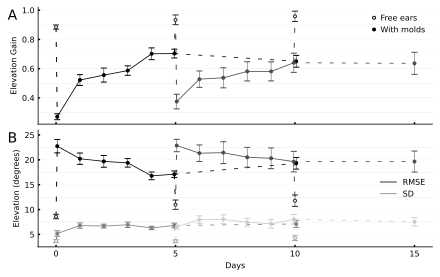
\includegraphics[width=13cm]{../Results/figures/ele_learning/ele_learning}}
\end{figure}
\begin{multicols}{2}
\noindent % prevent indent

\noindent \textbf{No difference between rates of adaptation to first and second earmolds}\\
To investigate possible effects of metaplasticity (i.e., an effect of the previous adaptation to earmolds 1 on the subsequent adaptation to earmolds 2) the rates of adaptation to the first and second earmolds were compared. To assess the rate of adaptation across participants independent of initial acoustical disruption caused by the earmolds, the increase in vertical localization accuracy during adaptation (performance on day 0 vs day 6) was divided by the initial decrease caused by the molds. Individual adaptation rates varied continuously and did not fall into discernable groups. No difference was found between the two sets of earmolds (two-tailed Wilcoxon signed rank test of Molds 1 vs Molds 2, Reduction of vertical RMSE from day 0 to day 6 divided by initial increase; Earmolds 1: 0.66 +/- 0.06 vs Earmolds 2:  0.74 +/- 0.09, p = 0.413). Individual adaptation performance with the first set of earmolds was positively related to adaptation performance with the second set of molds, although not significant (R = 0.47, p = 0.142). No correlation was found between vertical spectral information of the earmolds in the 3.7 – 12.9 kHz band and adaptation performance.\\

\noindent\textbf{Adaptation was generalizable}\\
To rule out the possibility of participants memorizing location-specific spectral features of the training stimuli in the localization test, the test was repeated with a subset of six participants on the last day of each adaptation period using stimuli of random spectral content (USOs). The effect of USO stimuli on vertical localization error did not differ between adapted earmolds and free ears indicating that generalizable perceptual learning had taken place (Friedman test; differences in vertical RMSE between pink noise and USO localization across conditions; Ears free: -0.38 +/- 1.82, Earmolds 1: 2.5 +/- 0.46, Earmolds 2: -0.15 +/- 0.45, p = 0.135).\\

\noindent\textbf{No aftereffect on free ears localization performance after mold removal}\\
Previous studies reported the absence of an aftereffect on localization performance with free ears after adaptation to new spectral cues for sound localization (Hofman 1998, Trapeu and Schönwiesner 2015). To confirm these findings, free ears localization accuracy was measured immediately after mold removal at the end of each adaptation period. 
No aftereffect was present for elevation gain but. An increasing impact on participants’ vertical localization accuracy with their native ears was observed after each adaptation period (see Fig. 1 B, one-tailed Wilcoxon signed rank test, vertical RMSE; free ears baseline vs free ears day 5: p = 0.002, free ears baseline vs free ears day 10: p = 6x10-4). \\



%%%%% spectral behavior %%%%%%%
 \noindent\newpage\textbf{Free ears localization accuracy was not explained by VSI or spectral strength}\\
Vertical spectral information and spectral strength was computed in 5 octave bands between 4 and 16 kHz (4–8 kHz, 4.8–9.5 kHz, 5.7–11.3 kHz, 6.7–13.5kHz, 8–16kHz) from sets of DTFs obtained with and without molds. As previously reported by \citet{trapeau_fast_2016}, VSIs of participants’ free ears varied among frequency bands (Kruskal-Wallis test, p = 8x10-3) and peaked in the 5.7 – 11.3 kHz band [Fig 5]. When comparing VSIs in this band with participants’ initial vertical localization accuracy, only vertical SD was significantly correlated (Spearman correlation of free ears VSI and vertical SD: R = - 0.55, p = 0.031). No correlation was found between spectral strength and behavioral metrics in this band. \citet{middlebrooks_individual_1999} reported a systematic variation in the frequencies of spectral features among individuals’ DTFs within the 3.7 – 12.9 kHz band. To account for the inter-individual differences in the distribution of spectral information across octave bands in the present data, behavioral measures were additionally compared to spectral features in this range of frequencies. Here the relation between participants’ free ears VSI and vertical localization accuracy was in the predicted direction, although not significant (Fig 5 A, Spearman correlation of free ears VSI and vertical RMSE: R = - 0.39, p = 0.151).\\

\noindent\textbf{Differences between first and second mold VSI dissimilarity to free ears}\\
Silicone molds were fitted with the aim of achieving consistent reduction of vertical localization performance across subjects and earmolds. To achieve this, stronger alterations in morphological features of the outer ears became necessary for the second set of molds compared to the first set. Consequently, differences between DTFs with molds and participants’ free ears were larger for the second set of earmolds (Wilcoxon one tailed signed rank test, VSI dissimilarity in the 3.7 – 12.9 kHz band, ears free and earmolds 1:  0.56 +/- 0.06 vs ears free and earmolds 2: 0.72 +/- 0.07, p = 0.002).\\

\noindent\textbf{Effects of acoustic dissimilarity between free ears and earmolds on localization accuracy}\\
To investigate whether acoustic and behavioral effects of the earmolds were related, the VSI dissimilarity between DTFs in the 3.7 – 12.9 kHz band with and without molds was compared to the decrease in participant’s localization performance after insertion of the earmolds. A trend of increasing vertical RMSE for larger acoustic differences was found for the first set of earmolds (Fig 5 B, Spearman correlation of vertical RMSE in the first test with molds compared to free ears and VSI dissimilarity: R = 0.38, p = 0.175). The relation between acoustic differences and behavior was still visible on the last day of the adaptation period (Fig 5 C, Spearman correlation of vertical RMSE in the last test with molds compared to free ears baseline and VSI dissimilarity: R = 0.38, p = 0.185). No such trend was found for vertical localization and VSI dissimilarity between free ears and the second set of molds (Spearman correlation of vertical RMSE in the first test with molds compared to free ears baseline and VSI dissimilarity: R = - 0.07, p = 0.832). Because initial vertical localization accuracy with the second earmolds could additionally depend on acoustic similarities to the previously learned set, differences in localization performance between the final test with earmolds 1 and the initial test with the earmolds 2 were compared to the VSI dissimilarity between both molds. A trend was found of increasing vertical error with greater acoustic dissimilarity between the first and second set of earmolds (Fig 5 D, Spearman correlation of vertical RMSE in the first test with second molds compared to last test with first molds and VSI dissimilarity: R = 0.29, p = 0.385).\\
